\chapter{Cross-session memory, raw traces, and compaction policies}\label{cross-session-memory-raw-traces-and-compaction-policies}

One of my own memory systems rebuilds its entire derived layer whenever the schema version changes. Nothing in that layer is migrated in place. Three append-only tables, holding lessons, memory events, and provenance events, cross the rebuild boundary through mechanical export and import, and everything else is recomputed from the work record it came from. The arrangement is deliberately inconvenient, and it comes with no comparative evidence that it outperforms a system that rewrites its memory as it goes.

The reason for the inconvenience has been measured elsewhere. Zhang (\href{https://arxiv.org/abs/2605.12978}{2026}) studied memories that language models update continuously and found that they degrade. A production account of Slack's context management described the same general shape. The Agentic Context Engineering synthesis (\href{https://arxiv.org/abs/2510.04618}{2025}) names two of the degradation modes, context collapse and brevity bias. Each rewriting pass optimizes a representation that is already the product of an earlier optimization. Deletion and distortion therefore accumulate without any explicit destructive operation, and routine maintenance damages the evidence.

I treat the complete chronological record of a session's inputs, actions, outputs, and state changes as the ground truth for cross-session memory. I call that record the raw, or episodic, trace. Everything derived from it must remain rebuildable. Observed query and task failures, rather than anticipated ones, determine when the storage and compression layers deserve more complexity.

The evidence base for this chapter is thin. Six items support its three design entries. Only two of the six are strong, and five are explorer-class syntheses rather than controlled experiments. The storage recommendation has no strong item at all and remains contested among practitioners. I therefore use this evidence to define architectures and measurement decisions. It supplies no defensible retention period, retrieval threshold, or compression ratio.

\section{Preserve the evidence before deriving the memory}\label{preserve-the-evidence-before-deriving-the-memory}

Continuous rewriting can leave the latest stored record without evidence that earlier versions contained. Support for this failure mechanism comes from one explorer-class study the evidence audit retained as strong, one directional synthesis, and the Slack production account named alongside them. The directional synthesis is Agentic Context Engineering (2025). The evidence audit records no quantitative result behind it, and it therefore supports the direction of the practice only. No controlled comparison of storage architectures is on record.

I therefore separate the immutable source record from every summary or fact derived from it. Material removed by an earlier rewrite cannot be recovered from the latest rewrite. A further pass may produce a better summary of the remaining text, but it has no observation from which to reconstruct what disappeared. The system has crossed a recovery boundary without marking the crossing. Treating each rewrite as a new authoritative state hides that loss behind a successful update.

An immutable raw layer changes the failure mode. The store appends the original session events and does not ask a model to modify them. A separate process reads those events and produces a summary, a profile, or a collection of extracted facts. I call that output the distillate, meaning a derived representation built from the source record for later use. When the distillate omits material from the source record, the omission is a retrieval or consolidation defect that can be repaired from preserved evidence.

The architecture has two ownership rules. The recorder owns fidelity to what happened, including ordering, identity, and state references. The distiller owns one interpretation of that record for a stated retrieval purpose. A summary may say what the system believed about a user, while the trace records which statement produced that belief, when it arrived, and what later event contradicted it. Collapsing the two roles into one mutable record converts an inference into history.

Rebuildability follows from that separation. Every derived item carries provenance back to the trace events that produced it and to the version of the extraction or summarization rule that interpreted them. When the schema changes, the system constructs a new derived store from the raw record. It does not ask a model to translate each old conclusion into a new conclusion in place. Parallel rebuilds also let an operator compare the old and new distillates before switching readers to the new version.

\begin{verbatim}
recorder
    -> inputs + actions + outputs + state changes
        -> complete chronological raw, or episodic, trace
           [ground truth: ordering + identity + state references]
                |
                v
distiller -> stated retrieval purpose -> derived store
                |
                +-> provenance -> trace events
                +-> version of extraction or summarization rule

schema changes
    -> raw record -> new derived store

earlier rewrite removes material
    -> latest rewrite cannot recover it
\end{verbatim}

The artifact here is the replayable trace from Chapter 9, used for a second purpose. In recovery, the trace reconstructs execution after a crash. In memory, it reconstructs a representation after that representation proves incomplete or wrong. The requirements overlap, but memory adds access patterns, retention decisions, and user-facing correction obligations that execution replay alone does not settle.

Consider a coding agent that learns three things during a repository investigation. An interface was renamed. A compatibility wrapper remains for one release. One service still calls the wrapper during rollback. A concise summary may retain the rename and the wrapper while dropping the rollback dependency as a low-frequency detail.

Weeks later, an incident task asks whether the wrapper can be removed, and a memory query against the summary returns a confident but incomplete answer. With the raw trace preserved, the system can respond in several defensible ways. It can retrieve the original observation directly. It can rebuild the facts under a schema that represents rollback dependencies. It can show the user that the current summary has no coverage for the question. Without the trace, the only available repair is another model-generated guess.

Continuous rewriting also confuses time. Suppose an early session records that a service owner is Priya. A later session records that ownership moved to Luis. A third task then asks who approved a decision made between those two dates. A profile optimized for the current owner may erase Priya entirely, while preserving both events lets the derived layer represent succession, validity intervals, or uncertainty across time.

This temporal case points to a design the companion catalog develops separately. A memory can supersede a claim for current use while retaining the earlier version for questions about the past. Work on temporal knowledge-graph memory, from Kim et al.~(\href{https://arxiv.org/abs/2408.05861}{2024}), is part of the support. The recommendation of two time axes, one for when a fact was true and one for when the system learned it, is practitioner-weighted rather than a measured result of that work, and it remains directional. The raw event order supplies the observations. The derived schema still has to decide how a claim becomes current, obsolete, or disputed.

Immutability does not mean public access or indefinite retention. Raw traces can contain credentials, personal attributes, proprietary code, and conclusions that later prove false. Their value as recovery material increases the damage from an access-control failure. I classify the raw layer as sensitive source material, restrict writers to append operations, encrypt it under a stated retention policy, and log every reader that crosses the boundary.

Deletion has to follow provenance in the other direction. If a user or a policy requires removal of a raw event, every summary, profile, embedding, cache entry, and graph edge derived from it becomes suspect. A deletion process that removes only the transcript leaves the more convenient copies intact. The system needs a mechanical way to find the affected derivatives, invalidate them, and rebuild what remains from authorized source material.

Forgetting is therefore part of the architecture, and it is the least-measured part of the memory stack in the evidence available here. A system may demonstrate that it retrieved retained facts without testing whether deleted or superseded facts still reach generation through a summary, a cache, or a model-produced profile. Deletion propagation and stale-claim retrieval should therefore be measured separately from task success. A task can succeed while a deleted fact is still shaping the answer.

Retention has a boundary the recovery argument cannot override. Some systems cannot lawfully or safely keep complete traces. Others should not keep them, because the likely harm exceeds their diagnostic value. In these settings, the raw layer may need field-level redaction, a shortened retention window, content-addressed references to separately governed artifacts, or deliberate noncollection. The design requirement is to make each loss explicit and testable. An already compressed record cannot serve as the raw recovery boundary.

\emph{Companion-site aside, thin support:} Persisting the repository regions an agent has already explored may prevent repeated discovery work across sessions. The idea rests on one directional source, from Pan et al.~(\href{https://arxiv.org/abs/2507.19942}{2025}). Whether it reduces redundant retrieval without also preserving stale interpretations should therefore be tested.

\emph{Companion-site aside, thin support:} Durable project state persisted across crashes and context loss in the long-horizon engineering system Chen (\href{https://arxiv.org/abs/2604.13018}{2026}) evaluated. That result is a directional reason to hand off artifact references between agents. No controlled comparison against transcript-summary handoff is on record, and the fidelity advantage over a summary therefore remains an inference. The receiving agent also needs a way to verify artifact identity, permissions, and version.

\section{Make the storage system earn its complexity}\label{make-the-storage-system-earn-its-complexity}

At a new agent project's architecture review, the design already contained a vector database and a knowledge graph. The query log was empty. Nobody had asked the system a question yet, and the retrieval architecture had already been settled.

The support for arguing against that default is directional, practitioner-weighted, and contested. It comes from three explorer syntheses and no strong item. Menschikov (\href{https://arxiv.org/abs/2506.17001}{2025}) compared knowledge-graph memory against lighter substrates in a personal-AI setting. Wolff and Bennati (\href{https://arxiv.org/abs/2601.07978}{2026}) compared cost against accuracy, and the evidence audit classifies that comparison as directional with no quantitative result behind it. Yang (\href{https://arxiv.org/abs/2602.05665}{2026}) surveyed graph-based agent memory, and that survey is the counterweight to the position taken here rather than support for it.

A practitioner argument that knowledge graphs are the wrong abstraction for agent memory runs alongside those papers, with no study behind it. Together these establish a presumption in favor of simpler infrastructure. They do not establish that relational storage wins across workloads.

I begin the decision with the corpus the agent records: session transcripts, tool observations, decisions, outcomes, and the provenance connecting derived facts back to those events. A relational database can store those records with stable identifiers, explicit time fields, access controls, and transactional deletion. Full-text search supplies an inspectable first retrieval path. The operator can see the query, the matched terms, the filters, and the returned rows without first interpreting a learned similarity score or a model-extracted edge.

This starting point is deliberately modest. It handles exact identifiers, quoted phrases, error text, names, paths, and combinations of structured filters with lexical search. It also exposes its own failures. If a user asks for ``the outage caused by stale ownership data'' while the trace says ``the on-call mapping lagged the transfer,'' lexical retrieval may miss the connection. This miss is evidence for a semantic retrieval lane, provided such mismatches recur in representative work.

Vector retrieval adds that lane by comparing learned representations of the query and the stored text. The extra machinery may be justified when users regularly describe the same event in different language, when terminology changes across teams, or when the useful passage shares a concept but few tokens with the query. It also introduces an embedding model whose version and chunking choices change the representation. The additional index needs its own update and deletion path. I assess those costs against observed lexical misses rather than against anticipated ones.

A knowledge graph makes a different promise. It represents entities and relations. The system can therefore traverse a question such as which services depend on a library owned by a team whose runbook changed after an incident. When relationships are the object of retrieval and multi-hop questions recur, the schema and maintenance cost of that representation can be justified. Similarity search is not a reliable substitute for explicit traversal when the answer depends on a chain of named relations.

The graph obtains those relations through an extraction pipeline. A model reads an event or a summary, decides which entities exist, resolves their identities, and emits edges. Each of those decisions can invent content, merge distinct entities, split one entity into several, or assign a relation the trace did not state. A graph can then return a mechanically correct traversal over semantically wrong edges, which makes the answer look better supported than its evidence warrants.

High-degree entities create a separate scaling problem. Common concepts such as production, a central platform team, or a widely used library can become hubs connected to much of the store. Queries through those hubs expand rapidly and return weakly related paths. The operator has to bound queries with relation constraints and temporal filters, and the pipeline has to prune weak edges and repair entity identities. Graph construction then becomes an ongoing information-quality program rather than a one-time schema decision.

The two additions solve different failures. A vector index addresses lexical mismatch. A graph addresses repeated relational traversal. Combining them may serve a workload that needs both, but the combination also compounds the provenance, synchronization, access-control, and deletion obligations. The design record should name which representative queries each component answers and which observed failures made the simpler path inadequate.

The decision has the same shape as Chapter 12's repository-index choice, but the corpora differ. Chapter 12 concerned how an agent indexes a repository that already exists. Here the corpus is the agent's own experience, and the extraction step may create entities or relations that were not present in the source. This difference raises the cost of an opaque derivation error.

Local-deployment claims need the same scrutiny. A memory framework may keep its database on a workstation while sending extraction or embedding requests to a remote model. Another may require a cloud key for the advertised default path even though its storage package is open source. I inspect the effective dependency graph, including model calls, embedding services, telemetry, background synchronization, and credential flow, before classifying a system as local.

Governance can change the preferred substrate before retrieval quality does. A relational transcript store may fit existing backup, audit, residency, row-level access, and deletion controls. A managed vector service might satisfy the same requirements with less operational effort in another organization. A graph may expose sensitive relations that no single source event revealed. Storage cost alone cannot decide among systems that create different privacy and accountability surfaces.

The comparison also has to separate correctness from performance. A full-text query that returns no relevant record has a retrieval-correctness problem even when it completes in milliseconds. A graph query that finds the right path but takes too long under hub expansion has a performance problem. A vector result that is useful but cannot be traced to an authorized source has a governance problem. Collapsing all three into `memory quality' hides which component has to change.

I use a small query set before adding infrastructure. It includes ordinary lookups, paraphrased requests, time-bounded questions, deletion checks, and the relational questions that prompted the discussion. For each query, I record whether the relevant evidence was retrieved, which irrelevant records displaced it, how the answer traces back to source events, what the operation cost, and whether the access policy held.

I draw this set from real tasks and failures, and I write it down before any candidate store is compared. Examples chosen after seeing which store handled them would favor that store, for the same reason Chapter 2 requires a task-exclusion rule to be declared before the outcomes are inspected.

The decision stays reversible while the raw layer remains independent. A vector index can be rebuilt from authorized transcript segments. A graph can be regenerated under a revised extraction schema and compared with its predecessor. If either system becomes necessary, it joins the derived layer and leaves the source intact. The recovery boundary remains intact while the retrieval architecture becomes more specialized.

A simple store can also be a false economy. Repeated lexical misses can force users to restate questions, cause the agent to proceed without prior evidence, and consume review time. Repeated manual joins across records can conceal relations the workload depends on. The presumption for simplicity expires when measured query failures and operating constraints show that the initial system cannot answer the work.

The opposite failure is easier to miss, because the system looks sophisticated while it fails. A graph built for future questions can make schema repair, entity reconciliation, and edge pruning the dominant memory task before any production query uses a traversal. A vector lane can accumulate embeddings whose source text has been deleted or superseded. Those maintenance costs belong in the same evaluation as the retrieval gains.

Scheduled consolidation into typed, pruned records can reduce query-time work once the types correspond to recurring retrieval needs. Scheduling changes when interpretation happens. It does not change the evidence boundary, because every consolidated item still needs source provenance and a rebuild path. Consolidating on a timer before the types have stabilized moves speculative extraction into a batch job.

Product and decision context may also need to be stored separately from code search. Dillon (\href{https://arxiv.org/abs/2605.08112}{2026}) measured coding-agent decision compliance when recorded product, design, and engineering decisions were available to the agent, and that support is directional. Extending it to runbooks, ownership changes, rejected designs, and incident lessons is an inference, though each of those answers questions that repository structure cannot. Such material should be stored under explicit source and time semantics, and code search should stay scoped to the repository.

\emph{Companion-site aside, thin support:} Memory portability favors exportable events, explicit schemas, and provenance another system can audit. The support, from Munirathinam (\href{https://arxiv.org/abs/2606.01138}{2026}), is anecdotal. A portability claim should therefore be tested with an actual export and import. A feature claim in a product description is not a test.

\section{Tune compaction against failures}\label{tune-compaction-against-failures}

A reviewer opens a failed trace annotated under Chapter 10's protocol and finds that the first upstream error followed a condensed-history update. Compaction is the replacement of working history with a condensed representation so a run stays inside its context budget. A fixed summarization prompt looks like routine maintenance, and its error profile goes unmeasured. One policy may preserve goals while dropping constraints. Another may retain decisions but blur which tool observation supported them. A third may keep every apparent dependency and fill the effective context length with obsolete branches.

The evidence for treating compaction as a tunable artifact rests on one strong literature study, from Kang et al.~(\href{https://arxiv.org/abs/2510.00615}{2025}), covering app, office, and question-answering agents. It includes no coding-agent benchmark. Transfer to repository work therefore remains an inference. That study supports treating each policy as a candidate component whose omissions, distortions, and distractions can be observed on tasks rather than assumed.

Chapter 10's protocol asks the reader to grow the corpus toward one hundred diverse traces and to cluster it into five to ten failure classes, assigning the first upstream error in each run. Those counts are unmeasured starting recommendations. For compaction, I add a context label only when the preserved trace supports it. The label states whether necessary evidence was missing, retained with changed meaning, or present but obscured by irrelevant history. It also records the compaction version and points to the source events that should or should not have survived.

This label is an attribution judgment rather than a measurement. Chapter 10 requires a named human to sign any attribution that changes remediation or the interpretation of an evaluation, and a change to the compaction policy is exactly such a decision.

The label also prevents a common attribution error. A task can fail after compaction even when memory played no causal role. The repository may have changed, a tool may have timed out, or the agent may have ignored evidence that remained plainly available. I revise the policy only when the trace supports a counterfactual claim. The claim is that a different representation of the same prior history could have changed the relevant decision.

The first policies are therefore hypotheses. Before any failure corpus exists, I can specify structural rules such as retaining current goals, unresolved constraints, artifact identities, decision provenance, and contradictory observations. I cannot know their relative value for a particular workload. The early system should preserve the raw material, record which rule produced each condensed history, and avoid presenting an untested prompt as optimized.

Once failures accumulate, I change one policy element at a time. A rule might preserve the exact observation behind an unresolved dependency, distinguish superseded facts from deleted facts, or discard completed exploratory branches after their artifacts have been recorded. I then re-run paired repeats on the same tasks using the discipline from Chapter 1. The comparison measures task success and the context used, and token count remains a secondary resource measure.

A comparison of two compaction policies is subject to the run-to-run variance Chapter 1 describes. One run of each policy is one draw. A difference that stays smaller than the measured spread should therefore not justify replacing the incumbent policy.

The compatibility-wrapper case provides a concrete policy test. The raw trace records that one service still calls the wrapper during rollback, while the compacted history drops that observation. The agent recommends removal, and the reviewer marks the recommendation as the first upstream error, caused by missing context.

I revise one rule so that unresolved rollback dependencies retain their source observation, then rebuild the condensed history from the same raw trace. Paired runs on the same removal task show whether the agent now preserves the wrapper and uses the retained evidence. I accept the change only when task success improves without a new distraction failure on neighboring cases. Otherwise the policy stays a hypothesis.

Kang et al.~reported peak-token reductions of 26 to 54 percent alongside improved task success across three app, office, and question-answering benchmarks. They also reported gains of up to 46 percent for small-model agents when distracting context was removed. Under those experimental designs, less context coincided with better reasoning. Those results do not establish an expected reduction or an expected success gain for coding agents.

\begin{figure}
\centering
\pandocbounded{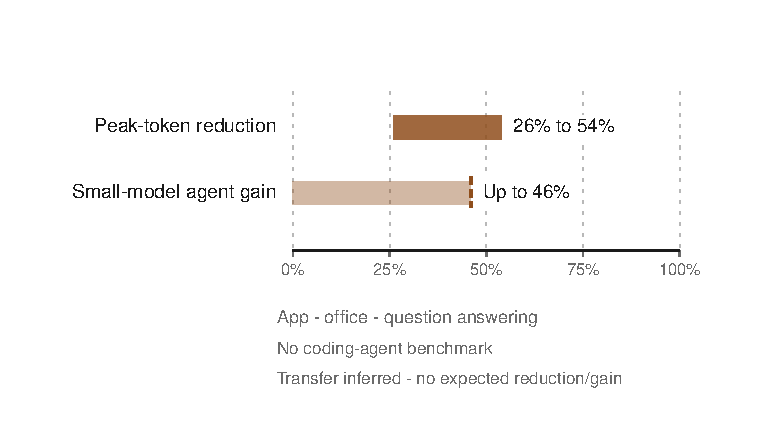
\includegraphics[keepaspectratio,alt={Across app, office, and question-answering agents, removing distractions cuts peak tokens by 26\% to 54\% and raises small-model success by up to 46\%; no coding-agent benchmark supports extrapolating either effect to coding agents.}]{figures/ch14-compaction-tokens.pdf}}
\caption{Across app, office, and question-answering agents, removing distractions cuts peak tokens by 26\% to 54\% and raises small-model success by up to 46\%; no coding-agent benchmark supports extrapolating either effect to coding agents.}
\end{figure}

The study covers app, office, and question-answering benchmarks, with no coding-agent benchmark; repository transfer remains an inference without an expected coding-agent reduction or gain.

The plausible mechanism is the work required to discriminate among records. A model presented with every prior attempt has to decide which constraints remain active, which observations are stale, and which abandoned branches should influence the next action. Irrelevant history competes with useful evidence for attention, and repetition can make an obsolete plan look current. Removing that material can improve correctness while also reducing inference cost.

Compression creates the inverse failure. A concise history may omit a rare constraint because it contributed few tokens or appeared only once. Frequency is a poor proxy when one low-salience fact controls whether a destructive action is permitted. The failure corpus reveals which details became decisive in actual investigations, and the policy can then preserve evidence by function rather than by apparent prominence.

Task success alone is still too coarse for diagnosis. I inspect whether the compacted context retained the decisive observation, preserved its qualification, and excluded material that had become irrelevant. A successful run can hide a damaged memory when the model guessed correctly or recovered through a tool call. A failed run can show a sound compacted context that the model then misused. Keeping those cases separate prevents the compactor from absorbing every downstream error.

Policy versions have to remain replayable. The same raw trace should produce the same condensed representation under a named policy and model configuration, or the rebuild has to record its nondeterminism explicitly. When retries occur, the system records whether they reuse the existing compacted state or rebuild from the raw trace. Otherwise a successful retry can conceal that the first and second attempts received different histories.

When a tuned policy stabilizes across new failures and held-aside traces from the same workload, its examples can train or distill a smaller model. This step changes latency and cost. It also creates another component to evaluate for semantic drift. The smaller model's outputs and downstream task behavior should therefore be compared against the accepted policy, and a route back to the larger compactor should stay open for cases it cannot handle.

The loop cannot start on the first day, because no local failure evidence exists yet. Borrowed rules can supply a safe initial hypothesis, and preserving raw traces can limit the cost of a wrong initial policy by making its derived representation rebuildable. Optimization begins only after the traces show which omissions and distractions cause errors. The dependency on Chapter 10's corpus is the reason compaction tuning comes after the rest of the retrieval and context architecture rather than before it.

\section{A staged protocol for recoverable memory}\label{a-staged-protocol-for-recoverable-memory}

Storage and retention decisions take effect in the first session. Revision of the compaction policy waits for Chapter 10's failure corpus. The sequence below separates the immediate controls from the evidence-dependent ones.

From the first run, I keep every permitted raw trace in inexpensive immutable storage, and I mark every summary, profile, extracted fact, vector, and edge as derived. I record provenance and policy versions before the derived layer becomes operationally important. I test retention limits and deletion propagation as part of the design, because a recovery boundary that violates its governance boundary cannot stay in service.

I start retrieval with a relational transcript store and full-text search. This start is a presumption drawn from contested, directional evidence, not a measured result. Observed local query failures justify moving beyond it. Before adding another lane, I write down the representative queries and the observed failures that would justify it: recurring lexical mismatch for vectors, recurring relational traversal for a graph. Operating cost, dependency exposure, deletion behavior, and access control belong in that decision.

I run the first compaction rules as hypotheses and keep their outputs reproducible from the raw trace. Once the Chapter 10 corpus contains context-caused failures, I revise the policy against those cases and re-measure task success on paired tasks. Token reduction is a capacity-planning number. It cannot substitute for evidence that the agent made better decisions.

Review capacity is a finite input, and it does not grow as the fleet grows. Part V takes up the people who answer for this work, and the interfaces and escalation rules built around their limited attention.

\section{Sources and evidence}\label{sources-and-evidence}

The evidence class and strength on each entry below come from its catalog record. Author-system cases in this chapter are narrative illustration and are not part of the evidence base.

\subsection{Preserve raw traces and distill separately}\label{preserve-raw-traces-and-distill-separately}

\begin{itemize}
\tightlist
\item
  explorer/strong: ``Useful Memories Become Faulty When Continuously Updated by LLMs'' (Zhang 2026), arXiv:2605.12978, with Slack production context management (InfoQ 2026-04) named in the same synthesis.
\item
  explorer/directional: Agentic Context Engineering, arXiv:2510.04618. Direction only.
\item
  Corroboration (narrative only): the author's memory system rebuilds its derived layer on schema changes and mechanically carries three append-only event tables across rebuilds.
\end{itemize}

\subsection{Use a light store by default}\label{use-a-light-store-by-default}

\begin{itemize}
\tightlist
\item
  explorer/directional: PersonalAI KG comparison (Menschikov), arXiv:2506.17001, with a contested practitioner thread named in the same synthesis. Direction only.
\item
  explorer/directional: Cost-and-Accuracy study (Wolff \& Bennati 2026), arXiv:2601.07978. Direction only.
\item
  explorer/directional (boundary citation): Graph-based Agent Memory survey (Yang 2026), arXiv:2602.05665. Cited as the counterweight, not support.
\item
  Corroboration: none on record.
\end{itemize}

\subsection{Optimize compaction from failures}\label{optimize-compaction-from-failures}

\begin{itemize}
\tightlist
\item
  lit/strong: Kang, M., et al.~(2025), ``ACON: Optimizing Context Compression for Long-horizon LLM Agents,'' arXiv:2510.00615 (Microsoft).
\item
  Corroboration: none on record.
\end{itemize}

\subsection{Companion-catalog records named inline}\label{companion-catalog-records-named-inline}

These are not part of this chapter's three taught entries. Each is named in the prose so a reader can follow the aside to its source, at the strength the record carries.

\begin{itemize}
\tightlist
\item
  explorer/directional: Temporal KG memory (Kim et al.), arXiv:2408.05861, carried by the companion record on modeling time explicitly. Supports the two-time-axes aside only.
\item
  lit/directional: Prometheus (Pan, H., et al.~2025), arXiv:2507.19942, carried by the companion record on persisting explored context. No figure quoted here.
\item
  explorer/directional: AiScientist long-horizon engineering (Chen 2026), arXiv:2604.13018, carried by the companion record on durable artifact handoff.
\item
  explorer/anecdotal: memorywire (Munirathinam 2026), arXiv:2606.01138, carried by the companion record on memory portability.
\item
  explorer/directional: Product context and coding-agent decision compliance (Dillon 2026), arXiv:2605.08112, carried by the companion record on the tribal-knowledge substrate. Its compliance figure is not used in the prose.
\end{itemize}

Author-system cases in this chapter are narrative illustration, not evidence.
